\documentclass[12pt,a4paper]{article}
\usepackage{amssymb,amsfonts,latexsym,amsmath,amssymb,epsfig,array,epsf,delarray,multicol}
\sloppy
\usepackage{mathabx}
\usepackage{mathrsfs}
\usepackage{tikz}
\usepackage{pgfplots}
\usepackage{wrapfig}
\pgfplotsset{compat=1.8}
\usetikzlibrary{arrows}
\renewcommand{\baselinestretch}{1.2}
\renewcommand{\arraystretch}{1}
\hoffset -0.5truecm
\oddsidemargin -.5cm
\topmargin 1cm
\parindent 0cm
\parskip -0.5cm
\textwidth 17.5cm \textheight 29.0cm
\newcommand{\ds}{\displaystyle}
\newcommand{\tc}{\makebox(0,0)[lc]{:}}
\newcommand{\mkbx}[1]{\makebox(0,0)[lc]{#1}}

\thispagestyle{empty}

\begin{document}
\newpage
\setlength{\unitlength}{1cm}
\begin{picture}(-2.0,1.5)(-2.0,1.5)
  \thicklines
  \put(-.5,6.6){\line(1,0){14}}  \put(-.5,2.5){\line(1,0){14}}
  \put(-.5,1.5){\line(1,0){14}}  \put(-.5,1.5){\line(0,1){5.1}}
  \put(13.5,1.5){\line(0,1){5.1}}\put(4.0,2.5){\line(0,1){3.1}}
  \put(4.0,3.5){\line(1,0){9.5}} \put(11.5,1.5){\line(0,1){1}}
  \put(11.55,1.5){\line(0,1){1}} \put(11.6,1.5){\line(0,1){1}}
  \put(13.45,1.5){\line(0,1){1}}
  \put(12.45,1.5){\line(0,1){1}}
  \put(10.45,1.5){
\includegraphics[width=1cm,height=1cm]{aruco.pdf}}
  \thinlines
  \put(-.5,5.6){\line(1,0){14} }
  \put(4.2,4.8){\mkbx{Name}}
  \put(4.2,4.3){\mkbx{Last Name}}
  \put(6.2,4.8){\tc}  \put(6.2,4.3){\tc}
  \put(1.6,5.25){\tc} \put(1.6,4.8){\tc}
  \put(1.6,4.35){\tc} \put(1.6,3.8){\tc}  \put(1.6,3.35){\tc}
  \put(1.6,2.8){\tc}
  \put(-.3,5.25){\mkbx{Code}}  \put(-.3,4.8){\mkbx{Acad.Year}}
  \put(-.3,4.35){\mkbx{Semester}}   \put(-.3,3.8){\mkbx{Date}}
  \put(-.3,3.35){\mkbx{Time}}  \put(-.3,2.8){\mkbx{Duration}}
  \put(6.5,7.1){\makebox(0,0)[c]{\large \bf  DGIST  \large Dept. of
  Physics \& Chemistry  }}
  \put(9.25,2.8){\makebox(0,0)[c]{TOTAL 120 POINTS}}

  %%%%%%%%%%%%%%%%%  PLEASE UPDATE EXAM INFORMATION  %%%%%%%%%%%%%%%%
  %                                                                 %
  \put(6.5,6.1){\makebox(0,0)[bc]{\bf GENERAL PHYSICS 2}}      %
  \put(6.5,5,7){\makebox(0,0)[bc]{\bf MIDTERM}}                   %
  %                                                                 %
  \put(1.8,5.25){\mkbx{{\em Bs103a}}}                              %
  \put(1.8,4.8){\mkbx {{\em 2025}}}                            %
  \put(1.8,4.35){\mkbx{{\em Spring}}}                                 %
  \put(1.8,3.8){\mkbx {{\em 12.06.2025}}}                           %
  \put(1.8,3.35){\mkbx{{\em 9:00}}}                               %
  \put(1.8,2.8){\mkbx {{\em 120 min }}}                             %
  %                                                                 %
  \put(9.25,3.2){\makebox(0,0)[c]{4 PARTS ON 9 PAGES}}          %
  %                                                                 %
  \multiput(.5,1.5)(1,0){4}{\line(0,1){1}}
  \put(-.45,2.45){\makebox(0,0)[tl]{\tiny 1. }}
  \put(0.00,2.45){\makebox(0,0)[tl]{\tiny ()}}
  \put(.55,2.45){\makebox(0,0)[tl]{\tiny 2. }}
  \put(1.00,2.45){\makebox(0,0)[tl]{\tiny ()}}
  \put(1.55,2.45){\makebox(0,0)[tl]{\tiny 3. }}
  \put(2.00,2.45){\makebox(0,0)[tl]{\tiny ()}}
  \put(2.55,2.45){\makebox(0,0)[tl]{\tiny 4. }}
  \put(3.00,2.45){\makebox(0,0)[tl]{\tiny ()}}
  %%%%%%%%%%%%%%%%%%%%%%%%%%%%%%%%%%%%%%%%%%%%%%%%%%%%%%%%%%%%%%%%%%%

\end{picture}
\mbox{\ } \vspace{-0.5cm} \mbox{\ } \\

\vspace{.5cm}
\vspace{.2cm}
\hspace*{6.54cm}
\raisebox{-0.8cm}{
\includegraphics[width=1cm,height=1cm]{aruco.pdf}}%
\hspace{0.2cm}%
\parbox[t]{3cm}{\scriptsize Use black or blue ball point pens to fill in
the circles.}
\begin{center}
  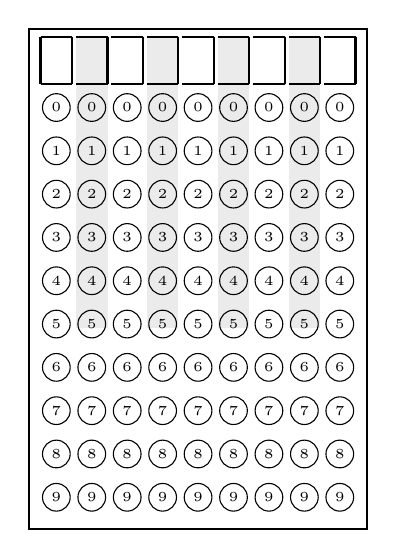
\begin{tikzpicture}[font=\small]
    % Define gradient colors
    \definecolor{lightblue}{RGB}{255,255,255}
    \definecolor{lightgray}{RGB}{235,235,235}

    % Create 9 columns for 9 digits
    \foreach \digit in {1,2,...,9} {
      % Determine background color (alternating)
      \pgfmathparse{mod(\digit,2)==1 ? 1 : 0}
      \ifnum\pgfmathresult=1
      \def\bgcolor{lightblue}
      \else
      \def\bgcolor{lightgray}
      \fi

      % Background rectangle for each column (tighter)
      \fill[\bgcolor] ({\digit * 0.45 - 0.2}, 0.5) rectangle ({\digit *
      0.45 + 0.2}, -3.2);

      % Hand-written digit box at the top of each column - only draw
      % left border for first box
      \ifnum\digit=1
      \draw[thick] ({\digit * 0.45 - 0.2}, 0.5) -- ({\digit * 0.45 -
      0.2}, -0.1);
      \fi
      % Draw top, bottom, and right borders for all boxes
      \draw[thick] ({\digit * 0.45 - 0.2}, 0.5) -- ({\digit * 0.45 + 0.2}, 0.5);
      \draw[thick] ({\digit * 0.45 - 0.2}, -0.1) -- ({\digit * 0.45 +
      0.2}, -0.1);
      \draw[thick] ({\digit * 0.45 + 0.2}, 0.5) -- ({\digit * 0.45 +
      0.2}, -0.1);

      % Create rows for digits 0-9
      \foreach \number in {0,1,2,3,4,5,6,7,8,9} {
        \begin{scope}[yshift={-\number * 0.55 cm - 0.4 cm}]
          % Bubble for each digit position with number inside (tighter spacing)
          \node[draw, circle, inner sep=1pt, minimum size=10pt] at
          ({\digit * 0.45}, 0) {\tiny\number};
        \end{scope}
      }
    }

    % Draw border box around the entire OMR sheet (much tighter)
    \draw[thick] (0.1, 0.6) rectangle (4.4, -5.75);
  \end{tikzpicture}
\end{center}

\vspace{0.13cm}
% \hspace*{9.81cm}
\includegraphics[width=1cm,height=1cm]{aruco.pdf}
% \begin{center}
%   \bf Closed notes, closed books. Attack all problems!
% \end{center}
\vspace{2cm}
\begin{center}
  \fbox{\fbox{\parbox{5.5in}{\centering
        \textbf{Please read the following instructions carefully.}
        \begin{itemize}
          \item You have 120 minutes to complete this exam. This
            question booklet contains 9 pages (including the cover)
            for the total. Check to see if any pages are missing.
          \item Answer the questions in the spaces provided after
            each question. If you run out of room for an answer,
            continue on the back of the page.
          \item Only standalone calculators are permitted. Devices
            with additional functionalities (e.g., internet access,
            text storage) are not allowed. Keep in mind that use of
            mobile phones or any other unauthorized electronic
            devices in the exam room is strictly prohibited.
        \end{itemize}
  }}}
\end{center}

\end{document}
